\newpage
\section{Hidden Surfaces}
In a complex scene where many objects can overlap it is important that polygons closer to the viewer \textbf{cover} the objects behind them. If faces are not drawn in the correct order unrealistic figures will appear.Respecting the proper order of primitives visualization is called \textbf{Hidden Surfaces Elimination}.\\
\begin{figure}[H]
  \centering
  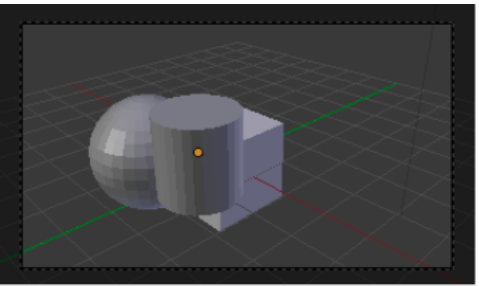
\includegraphics[width=.4\linewidth]{hiddensurfaces}
\end{figure}
When dealing with non-transparent object a technique called \textbf{Painter Algorithm} is applied : primitives are drawn in reverse order with respect to the distance from the projection plane : in this way,objects closer to the the view cover the oner further away.\\
In this figure above the drawing order is cube - sphere - cylinder.
There are cases in which the painter algorithm cannot be applied.
\begin{figure}[H]
  \centering
  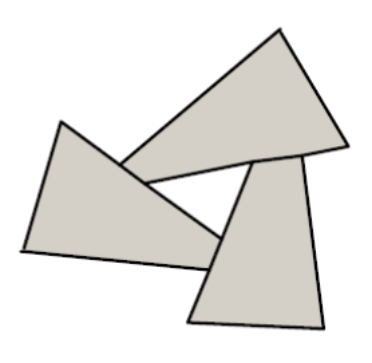
\includegraphics[width=.4\linewidth]{nopaint}
\end{figure}
In this case the primitives must be split so that is possible to find	a proper order of the considered pieces.
\begin{figure}[H]
  \centering
  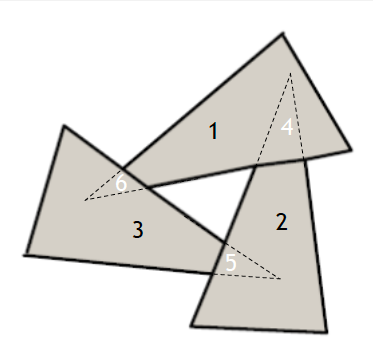
\includegraphics[width=.4\linewidth]{nopaintsplit}
\end{figure}
Three main algorithms are used for hidden surface elimination:
\begin{itemize}
\item \textbf{Back-face culling}\\
Allows identifying and excluding objects that belong to the back of an object
\item \textbf{Occlusion culling}\\
Excludes objects that fall completely behind others ( not covered in the course)
\item \textbf{Z-Buffering}\\
Allows to implement the painter algorithms without sorting the polygons by distance.
It is a per pixel based algorithm.
\end{itemize}
Z-Buffering alone is \textbf{enough} for hidden surface performance. However Occlusion and Back-face culling can increase the \textbf{performance}.

\subsection{Back-face culling}
This techniques allows to exclude objects that belong to the backside of a mesh simply considering:
\begin{itemize}
\item \textbf{Normal vectors}:\\
Can be stored either with the faces or computed on the fly if the vertices are ordered in a specific direction.
\item \textbf{Projection vectors}:\\
Depend on the projection type
\end{itemize}
\begin{figure}[H]
  \centering
  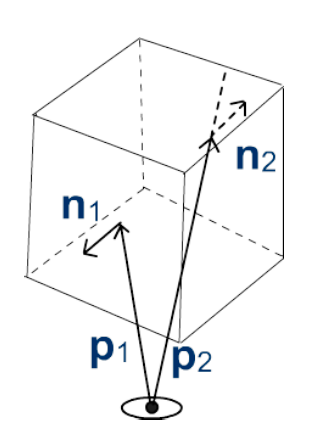
\includegraphics[width=.4\linewidth]{backface}
\end{figure}
A cube is encoded as a set of 12 triangles. All the triangles are obviously \textbf{planar} surfaces. Each triangle surface has its \textbf{normal} vector n ,directed outside. The projection rays are directed from the viewer to the object.
By performing a \textbf{scalar product} $p \cdot n$ we obtain:
\begin{itemize}
\item $p \cdot n < 0$ then the object belong to the \textbf{front}
\item $p \cdot n > 0$ then the object belong to the \textbf{back} and is occluded by
 the front faces.
\item $p \cdot n = 0$ then face is perfectly aligned with the projection rays and so it is seen at most as one single pixel
\end{itemize} 	
The normal vector :
\begin{itemize}
\item can be stored together with the face. This is a simple and fast solution but required more memory. Changing the position of the face must also result in a change in the normal vector.
\newpage
\item can be easily computed at run time from the vertices of the object if they are stored using a consistent order (eg.: clockwise). 
\begin{figure}[H]
  \centering
  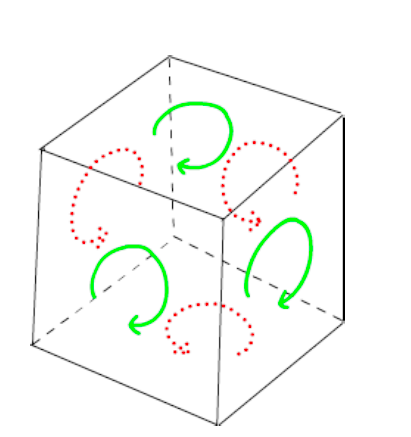
\includegraphics[width=.4\linewidth]{backfaceclock}
\end{figure}
The cross-product of two vectors is a vector that is perpendicular to the plane (direction is determined by the right hand rule). In triangles the normal vector can be computed starting from the difference of two vectors (identified by the vertexes) and then the cross product of the two differences is computed.
\begin{figure}[H]
  \centering
  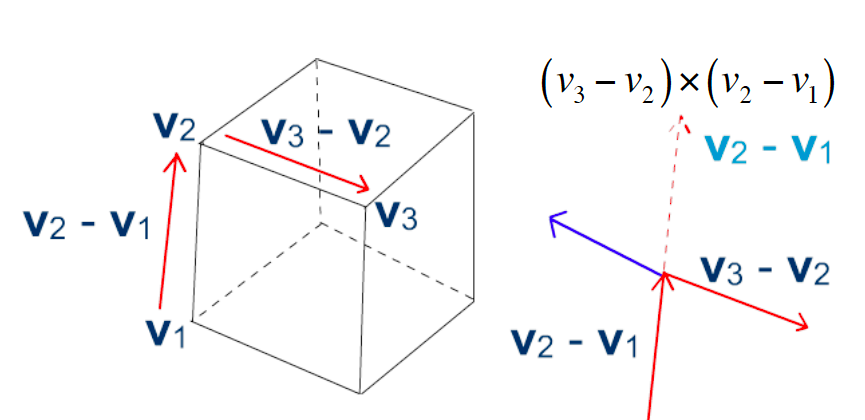
\includegraphics[width=.4\linewidth]{backfacecross}
\end{figure}
\end{itemize}
The projections rays:
\begin{itemize}
\item in \textbf{parallel} projection the vector p is \textbf{fixed} and corresponds to the direction of the projection ray.
\begin{figure}[H]
  \centering
  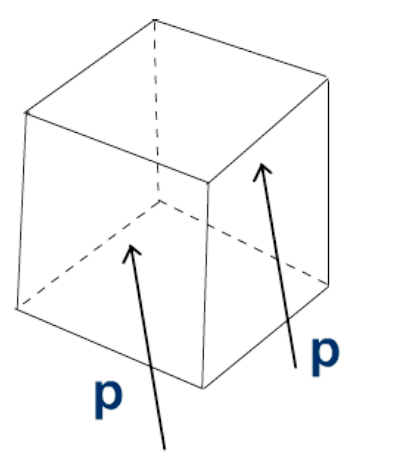
\includegraphics[width=.4\linewidth]{bfparallel}
\end{figure}
\item in \textbf{perspective} projection the vector p must be computed relative to one of the vertices ( planar faces means that any vertex is equivalent) and the center of projection O : $p= v-O$
\begin{figure}[H]
  \centering
  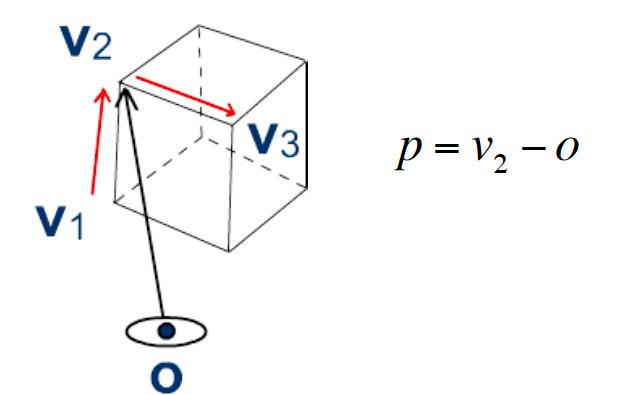
\includegraphics[width=.4\linewidth]{bfpersp}
\end{figure}
\end{itemize}
We must also take into account that scaling with \textbf{negative} values (central or planar mirroring) may invert the direction of the vertices. The sign to accept/reject a face must change accordingly.\\
To summarize :
\begin{figure}[H]
  \centering
  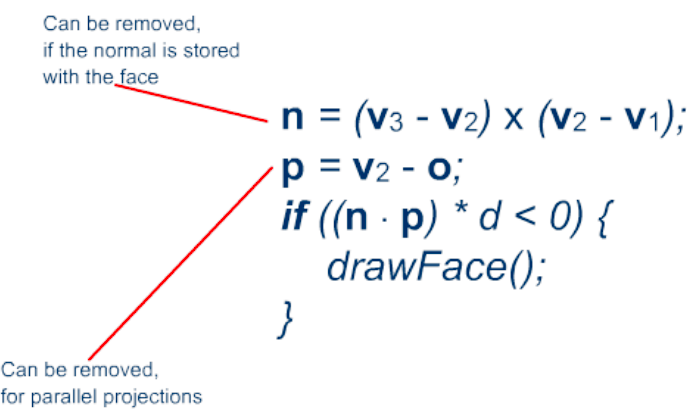
\includegraphics[width=.4\linewidth]{backfacesumm}
\end{figure}
Where d is a constant of +1 if we want to accept faces ordered clockwise or -1 if we want to accept faces ordered counter clockwise.\\
Back-face culling can be applied :
\begin{itemize}
\item \textbf{before} the world and view transformations.In this case the center of projection or the projection rays have to be mapped in the local space of the object by \textbf{inverting} the view and world transformations.
\item \textbf{after} the world and view transformations. In this case if the vector has been stored with the face then also the normal vector needs to be transformed.
\end{itemize}
Finally back-face culling cannot always be applied:
\begin{itemize}
\item in \textbf{non-2 manifold} objects ( where we can have holes or lamina faces). 
\item in \textbf{transparent} objects where the back face must be visible from the front face
\end{itemize} 
\begin{figure}[H]
  \centering
  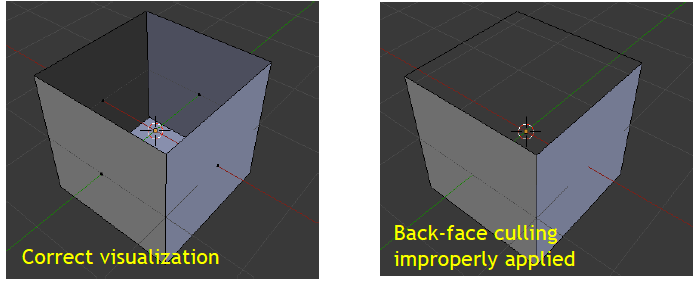
\includegraphics[width=.4\linewidth]{backfaceincorr}
\end{figure}
Usually engines separate non-2 manifolds from 2-manifolds for this reason.\\
Another special situation is when the camera is \textbf{inside} an object ( for example inside a room/box). In this case the normal is oriented in the wrong direction. When designing a scene this must be taken into account if back-face culling is applied : implementing this kind of situation without special adjustments means that the back-face culling algorithm hides the surface ( basically the camera shows objects behind a solid wall which he should not really see). 
\begin{figure}[H]
  \centering
  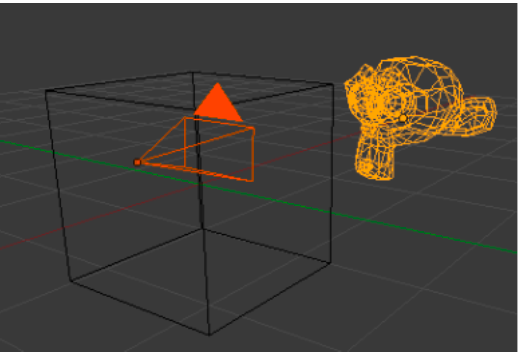
\includegraphics[width=.4\linewidth]{backfacewall}
\end{figure}
A solution to this is to create a room/skybox with the normal vectors pointing towards the \textbf{inside.}

\subsection{Z-Buffering}
Applies the painter algorithm to the \textbf{pixel} resulting from complete projection sequence rather than the faces of the objects drawn. This results in an extra memory area ( \textbf{z-buffer} ) that stores additional information for every pixel on the screen ( for an HD screen almost 2 million values so around 8MB!).\\
The algorithms draws all primitives on the screen that have passed \textbf{clipping} and \textbf{back-face culling} and tests whether to draw their corresponding pixels on screen.\\
For each pixel both the color and the \textbf{distance} from the observer are computed.The z-buffer stores the \textbf{distance} (i.e. the \textbf{z-coordinate}) for each pixel on the screen.
\begin{figure}[H]
  \centering
  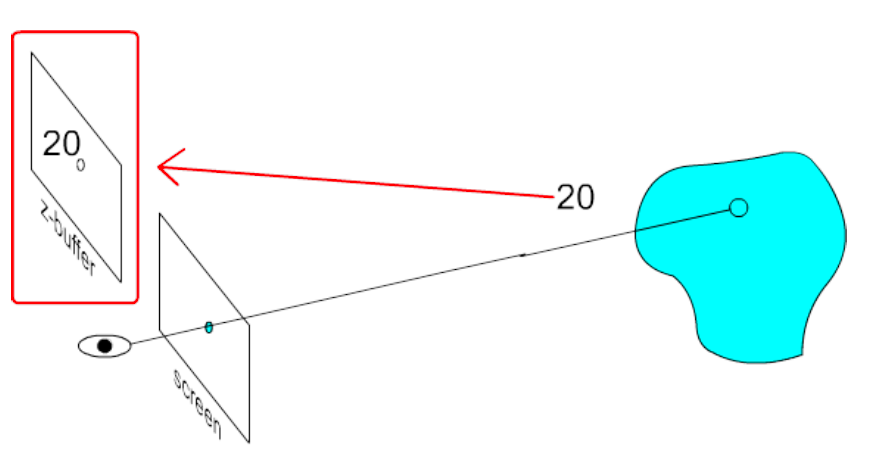
\includegraphics[width=.4\linewidth]{zbuff1}
\end{figure}
Then when a new objects is tested the algorithms checks ,pixel per pixel, if it is already in the buffer.If it is and the new distance is lower then it is \textbf{updated} in the z-buffer.
\begin{figure}[H]
  \centering
  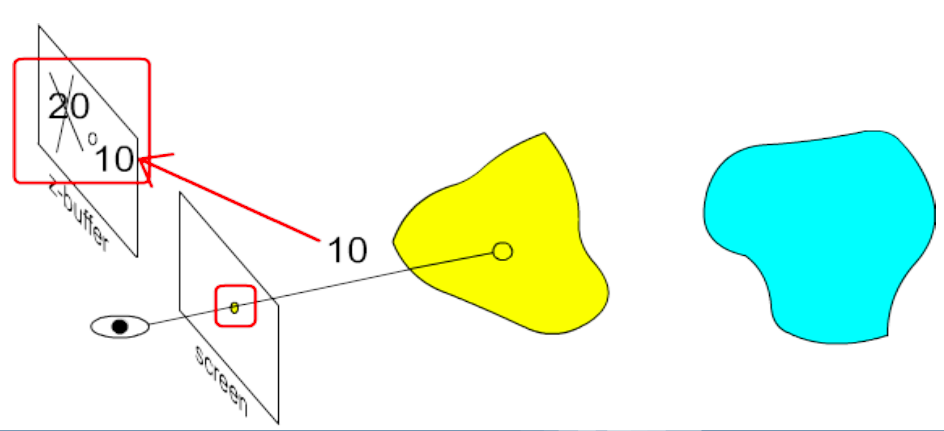
\includegraphics[width=.4\linewidth]{zbuff2}
\end{figure}
\subsubsection{Z-Buffering issues}
\begin{description}
\item[Issue 1]\hfill\\
This technique is very simple and solves all the hidden surface problems but it also computationally expensive. It not only requires to save the z-buffer area but also to compute all the \textbf{pixels} of the primitives. This is way back-face culling or occlusion culling \textbf{improve} the performance.
\item[Issue 2]\hfill\\
When dealing with triangles and their pixels also the z-coordinate must be interpolated : this is not always easy. \textbf{Normal screen coordinates} of x,y,z are in the range -1,1 and \textbf{pixel coordinates} are even more compressed for z in the range $z_n \in [0,1]$. 
\begin{figure}[H]
  \centering
  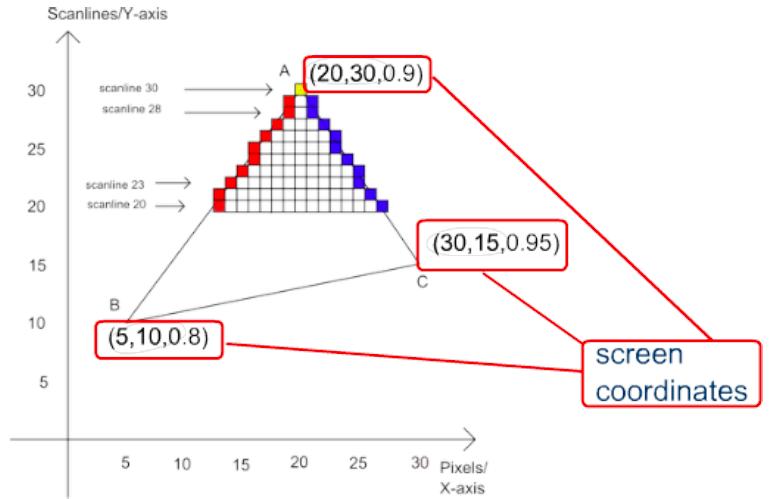
\includegraphics[width=.5\linewidth]{zbuffscreen}
\end{figure}
With these coordinates the vertices can be stored and from there via \textbf{interpolation} the corresponding pixels can be found. However the z-coordinate on screen has a \textbf{non-linear} behaviour : the distance between the lines becomes smaller as we move away from the plane and cannot be obtained by using interpolation in local/world/camera or clipping coordinates. The solution is to use the component $z_s$ of the \textbf{normalized screen coordinates} where $z_s = \frac{z_c}{w_c}$ is obtained from the clipping coordinates (see \textbf{perspective correct interpolation} with proof later on).
\item[Issue 3]\hfill\\
Another issue is \textbf{numerical precision} : the largest part of the $[0,1]$ range of the $z_s$ coordinates is used for the points that are very \textbf{close} to the projection plane (and not much used in the real scene)
\begin{figure}[H]
  \centering
  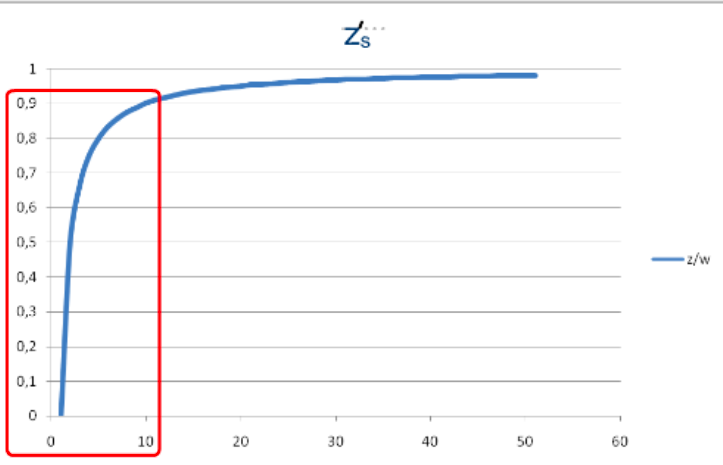
\includegraphics[width=.5\linewidth]{numprec}
\end{figure}
Since values a \textbf{discretized} we need more precision to store values that are further away otherwise a problem called \textbf{Z-fighting} occurs: when two almost co-planar figures are rendered the final \textbf{color} is determined by the round off error.
\begin{figure}[H]
  \centering
  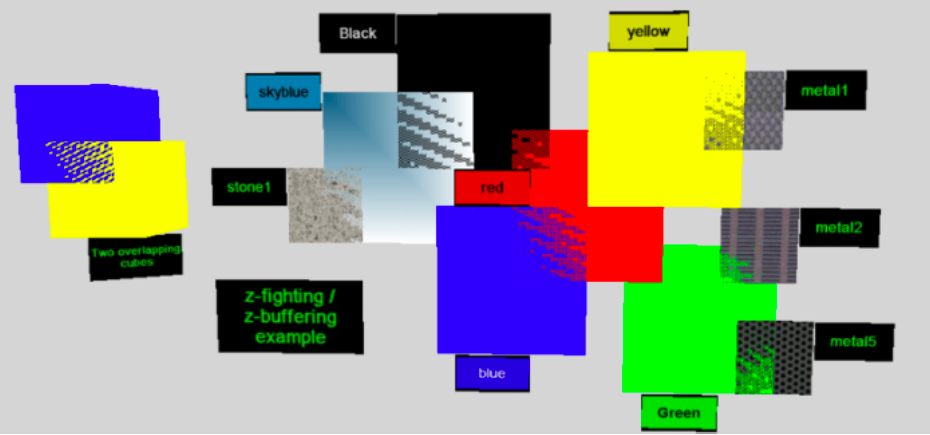
\includegraphics[width=.5\linewidth]{zfight}
\end{figure}
Since the $z_S$ coordinate is normalized with respect to the \textbf{near} and \textbf{far} planes these two parameters cannot be set to be arbitrarily small/large but must always be appropriate for the scene.
\end{description}

\subsubsection{Stencil buffer}
It is a technique similar to Z-buffer ,adopted to prevent an application to draw in some region of the screen.Again it is per pixel so an extra memory area (\textbf{stencil buffer}) is used to store data about each pixel. This kind of buffer is used to render for example head up displays in games like Wing Commander. More complex applications use the stencil buffer  to draw \textbf{shadows} and \textbf{reflections} in multi-pass rendering techniques.\\
\begin{figure}[H]
  \centering
  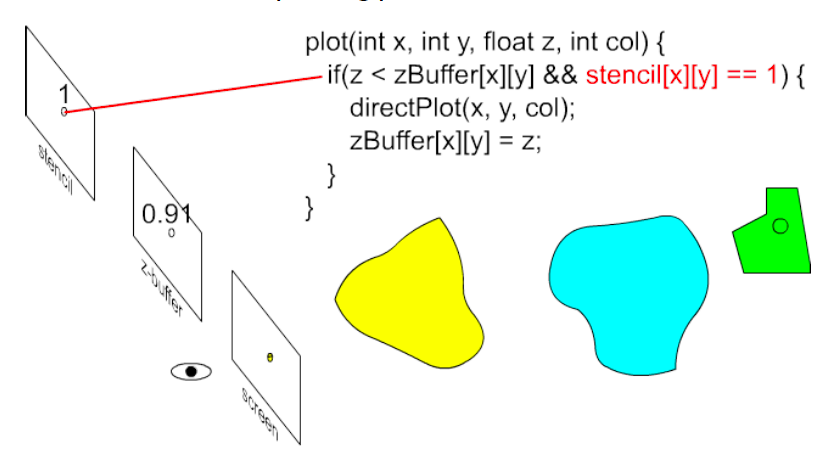
\includegraphics[width=.5\linewidth]{stencil}
\end{figure}
The buffer is a memory area that stores an integer information for each pixel (encoded at bit level). Usually binary values are stored :
\begin{itemize}
\item 1 the pixel must be drawn
\item 0 the pixel can be skipped
\begin{figure}[H]
  \centering
  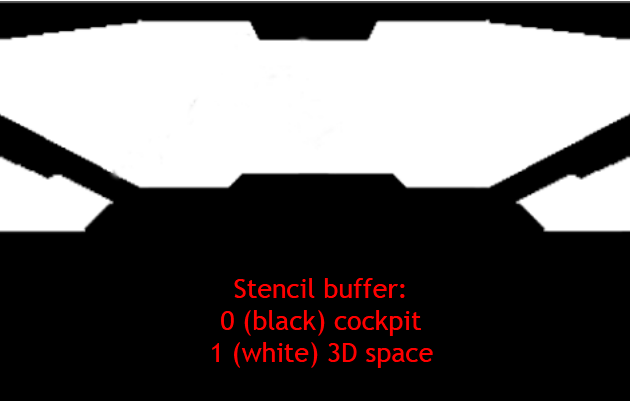
\includegraphics[width=.5\linewidth]{stencil2}
\end{figure}
But more complex encodings/scenarios can be used with the stencil buffer. 
\end{itemize}